\section{Frequentist Analysis}
\label{sec:frequentist}
\label{app:freq}
\emph{In short: the likelihood maximized for the two charges together gives $N_s=15{,}328\pm133$ and $\hat A=-0.0441$ with Minos intervals; $A=0$ is rejected at $5.2\sigma$ and the interval has nominal coverage in $1000$ bootstrap replicas.}
The Frequentist analysis estimates \Araw by maximizing the extended unbinned likelihood of Eq.~\eqref{eq:likelihood} with \texttt{iminuit}~\cite{iminuit}; the uncertainty and the test of $A=0$ come from the profile likelihood, the other parameters being nuisance parameters (Secs.~\ref{sec:freq_model}--\ref{sec:freq_ci}).

\subsection{Mass Model and Fit Strategy}
\label{sec:freq_model}
\label{sec:freq_simfit}
The common mass model of Sec.~\ref{sec:model} (Eq.~\eqref{eq:mixture}) was fitted on $[5100,5600]\,\MeV$: a Gaussian signal with mean $\mu$ and width $\sigma$ shared by the two charges and a double-exponential background with shape and yield of its own for each charge, twelve parameters as in the Bayesian fit, through \texttt{iminuit.cost.ExtendedUnbinnedNLL}; the minimization started from an unbinned fit of the sidebands (the window without $[5200,5350]\,\MeV$). The asymmetry was estimated in two ways: in the \emph{simultaneous} fit the two charges share $N_s^\pm=N_s(1\mp A)/2$ and $A$ is a parameter of the likelihood; in the \emph{separate} fits each charge was fitted alone (seven free parameters each) and $\Araw=(N_s^--N_s^+)/(N_s^-+N_s^+)$ was computed from the two yields. They give $-0.0441\pm0.0085$ and $-0.0442\pm0.0087$: sharing $\mu$ and $\sigma$ between a particle and its antiparticle is adequate, and the simultaneous fit, which gives the profile-likelihood interval directly, is the nominal one. It gives $N_s=15{,}328\pm133$ and $N_b=4{,}403\pm82$, against the Bayesian posterior medians $15{,}328\pm133$ and $4404\pm82$ (Sec.~\ref{sec:bayes_posterior}). The shapes were not tuned on this fit, and the alternatives are systematic variants (Sec.~\ref{sec:syst}). The nominal fit has $\chi^2/\mathrm{ndof}=160/88$ ($p=4.8\cdot 10^{-6}$) in $2\times50$ bins of $10\,\MeV$; a single exponential is rejected ($294/92$, $p=5.7\cdot 10^{-23}$)\appref{sec:validation_gof} because the background rises towards the lower edge of the window (Sec.~\ref{sec:data_mass}). The fit of the two charges is shown in Fig.~\ref{fig:freq_jointfit}.

\begin{figure*}[t]
\centering
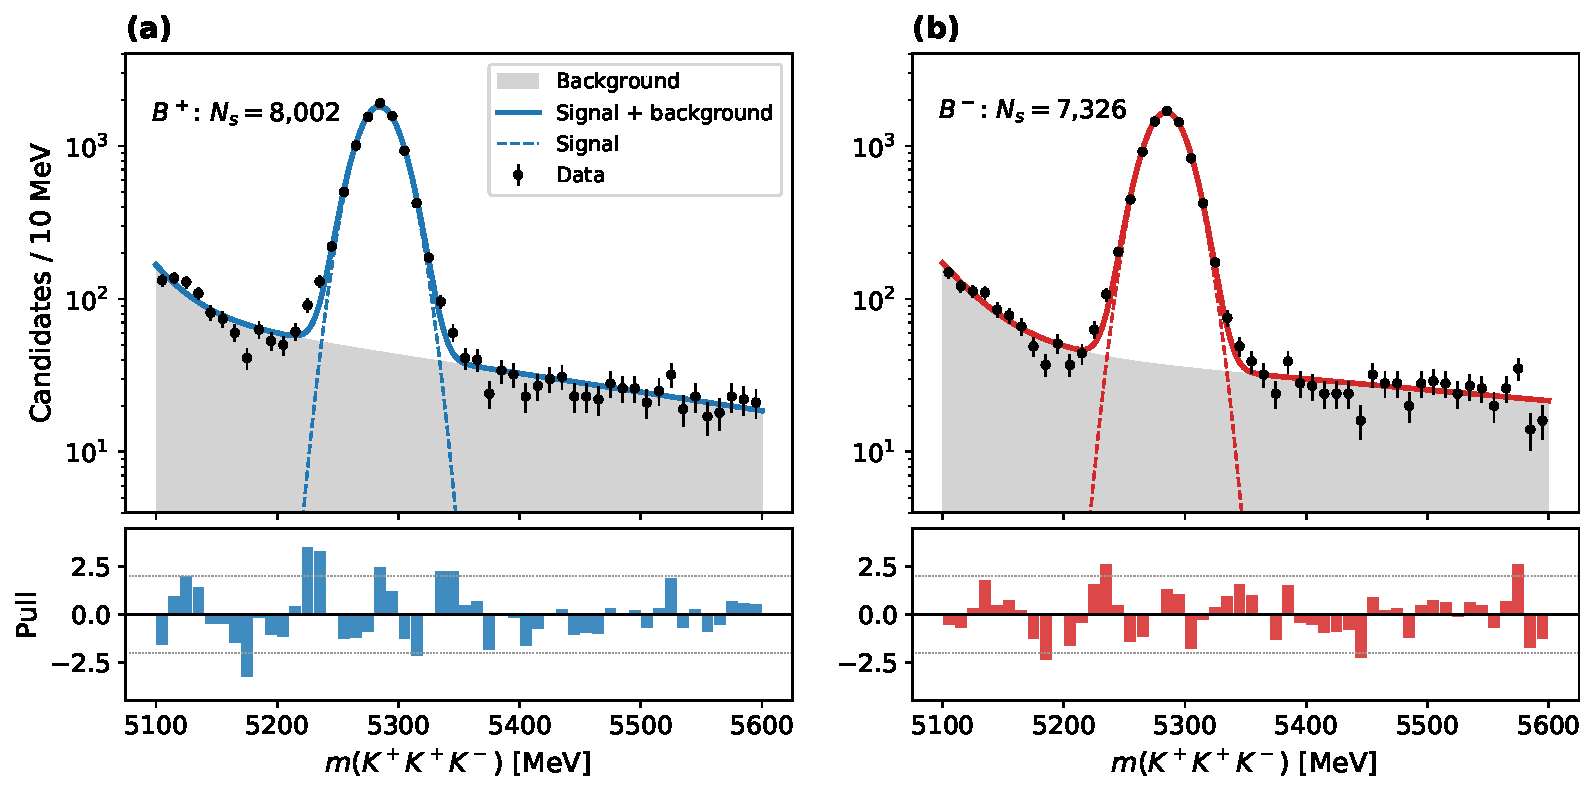
\includegraphics[width=0.95\textwidth]{figures/freq_jointfit.pdf}
\caption{Simultaneous fit of (a) $B^+$ and (b) $B^-$ in $10\,\MeV$ bins, logarithmic scale: data, signal (dashed), double-exponential background (grey) and their sum; below, the pulls $(n_i-\mu_i)/\sqrt{\mu_i}$ of the fit, with the $\pm2$ lines. The fitted signal yields are $8002$ and $7326$.}
\label{fig:freq_jointfit}
\end{figure*}

\subsection{Profile Likelihood and Confidence Interval}
\label{sec:freq_ci}
The maximum-likelihood estimate is $\hat A=-0.0441$ (Hesse uncertainty $0.0085$), with \texttt{MINOS}~\cite{minuit} intervals $68\%$ CI $[-0.0526,-0.0356]$ and $95\%$ CI $[-0.0607,-0.0275]$; the uncertainties are statistical only (the systematic one is in Sec.~\ref{sec:syst}). The profile likelihood ratio $q(A)=-2\log[L(A,\hat{\hat\theta})/L(\hat A,\hat\theta)]$, with the other eleven parameters re-minimized at each $A$ (\texttt{mnprofile}), is shown in Fig.~\ref{fig:freq_profile}; by Wilks' theorem~\cite{wilks} it follows a $\chi^2$ distribution with one degree of freedom at the true value of $A$, so the intervals are the sets $q\leq1$ and $q\leq3.84$. For the null hypothesis, $q(0)\simeq27$, $p=2.05\times10^{-7}$, $5.20\sigma$\appref{sec:appendix_freq}: no asymmetry is rejected, the counterpart of the Savage-Dickey test of Sec.~\ref{sec:bayes_factor} ($A=0$ at $5.2$ posterior standard deviations); the $p$-value is not the probability of $H_0$ and the Bayes factor depends on the prior width, but the conclusion is the same. The result agrees with the Bayesian one (Sec.~\ref{sec:bayes_posterior}: $-0.0443$, $68\%$ CI $[-0.0528,-0.0358]$), as expected with flat priors and $\sim2\times10^4$ events.

\begin{figure}[h]
\centering
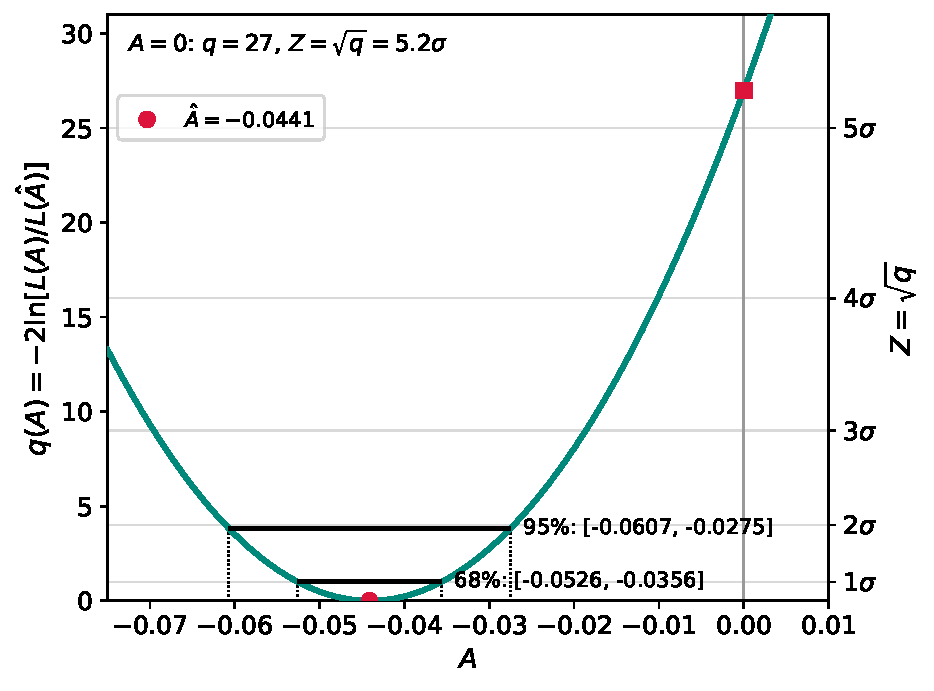
\includegraphics[width=\columnwidth]{figures/freq_profile.pdf}
\caption{Profile likelihood ratio $q(A)$ of the simultaneous fit, with the other eleven parameters re-minimized at each $A$ (right axis: $Z=\sqrt q$). The horizontal segments are the $68\%$ and $95\%$ Minos intervals ($q\leq1$, $q\leq3.84$); at $A=0$, $q\simeq27$, i.e. $5.2\sigma$.}
\label{fig:freq_profile}
\end{figure}

\subsection{Coverage of the Wilks Intervals}
\label{sec:freq_coverage}
Wilks' theorem is asymptotic, so the coverage was checked on the data with $1000$ bootstrap replicas of the $19{,}731$ candidates, refitting the nominal model on each (non-converged fits discarded); with $A_{\mathrm{true}}=-0.0441$, the $68\%$ interval of a replica contains it if and only if $q(A_{\mathrm{true}})\leq1$. The fraction is $68.4\pm1.5\%$ against $68.3\%$ nominal (Fig.~\ref{fig:freq_toys}). It agrees with the toy-MC check of the Bayesian interval ($65.0\pm3.3\%$, $200$ experiments)\appref{sec:bayes_toymc}; the two checks are not equivalent, since the Bayesian pseudo-datasets come from the fitted model (a closure test) while the replicas are resampled from the data and carry the features that the model does not describe, such as the signal tails\appref{sec:bayes_gof}.

\begin{figure}[h]
\centering
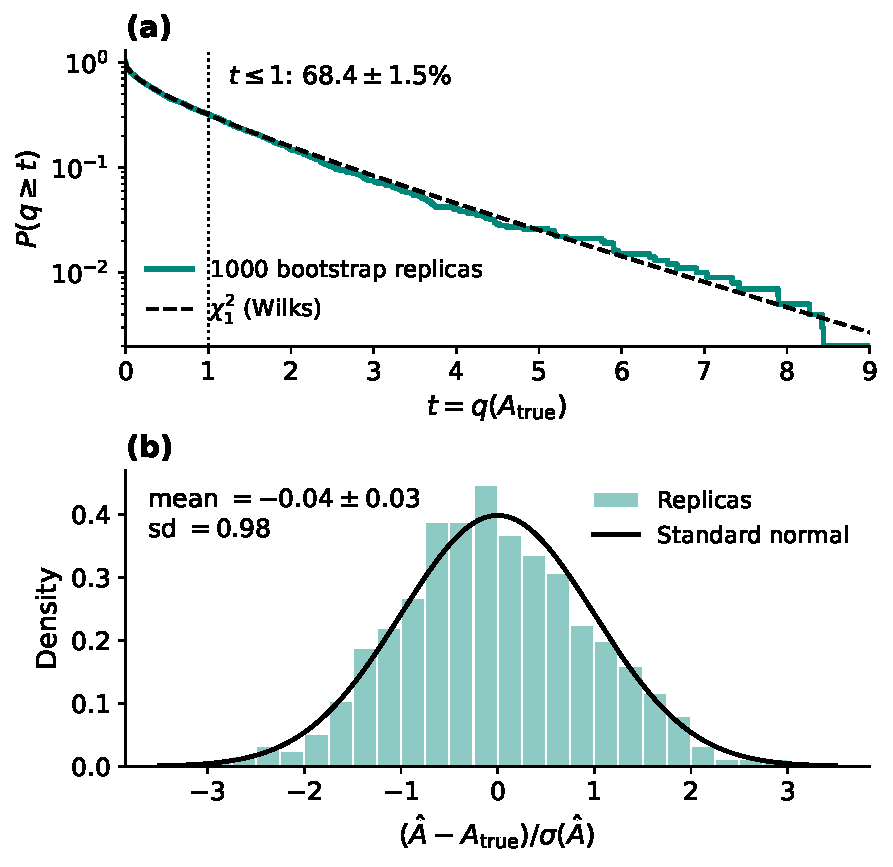
\includegraphics[width=\columnwidth]{figures/short_coverage.pdf}
\caption{Coverage check with $1000$ bootstrap replicas of the data. (a) Survival function of $t=q(A_{\mathrm{true}})$ against the $\chi^2_1$ distribution expected from Wilks' theorem; the dotted line is the $68.3\%$ limit ($t=1$). (b) Pulls $(\hat A-A_{\mathrm{true}})/\sigma(\hat A)$ of the replicas against a standard normal.}
\label{fig:freq_toys}
\end{figure}

\subsection{Hesse Uncertainties, Test of $A=0$ and Significance}
\label{sec:appendix_freq}
\emph{In short: the Hesse matrix is the inverse of the Fisher information, the test statistic is the profile likelihood ratio, and the significance is $Z=\sqrt{q(0)}$.}
\paragraph{Hesse uncertainties.}
For $n$ independent candidates the likelihood contains the information on the parameters $\theta$ through the Fisher information matrix, $I_{ij}=-E\big[\partial^2\ln L/\partial\theta_i\partial\theta_j\big]$. The information inequality (minimum variance bound) states that the variance of an estimator cannot be smaller than the inverse of $I$ (for an unbiased one), and the maximum-likelihood estimate reaches the bound asymptotically, where it is also unbiased and Gaussian~\cite{cowan}. The covariance matrix of the fit is therefore $V\simeq I^{-1}$ evaluated at the best-fit point, with the second derivatives of $-\ln L$ computed numerically: this is the Hesse matrix of \texttt{iminuit}, and $\sigma(A)=0.0085$ is the square root of the diagonal element of $V$ for $A$, which includes the effect of the eleven nuisance parameters. It assumes that $-\ln L$ is parabolic around the minimum. The Minos intervals do not: they follow the profile likelihood on each side of the minimum, and their agreement with the Hesse error ($-0.0085$, $+0.0085$) shows that the parabola is a good description here.

\paragraph{Test of $A=0$.}
The null hypothesis $H_0$: $A=0$ is tested against the alternative $H_1$: $A$ free, the other parameters being free in both. The test statistic is the profile likelihood ratio,
$q(0)=-2\ln\big[L(0,\hat{\hat\theta})/L(\hat A,\hat\theta)\big]=2\Delta\mathrm{NLL}$ (NLL: negative log-likelihood), large when the data disfavor $H_0$. For two simple hypotheses the likelihood ratio is the most powerful test of a given size, i.e.\ the one with the highest probability of rejecting $H_0$ when $H_1$ is true (Neyman-Pearson lemma~\cite{neyman_pearson}); the profile likelihood ratio is its extension to hypotheses with unspecified parameters, with no optimality guarantee in general. By Wilks' theorem~\cite{wilks}, under $H_0$ the statistic follows a $\chi^2$ distribution with one degree of freedom, the number of parameters fixed by $H_0$, whatever the number of nuisance parameters, so the $p$-value is $P(\chi^2_1\geq q_{\mathrm{obs}})$; this is the probability, under $H_0$, of a result at least as discrepant as the data, not the probability of $H_0$.

\paragraph{Significance.}
A $\chi^2_1$ variable is the square of a standard normal one, so $p=P(|N|\geq\sqrt{q})$ and the significance quoted is $Z=\sqrt{q(0)}$ ($q\simeq27$, $p=2.05\times10^{-7}$, $Z=5.20$). This is a two-sided convention: the one-sided one, $Z=\Phi^{-1}(1-p)$, applied to the same $p$ would give $5.06$. For a parabolic likelihood $\sqrt{q}$ coincides with the Hesse significance $|\hat A|/\sigma(A)=5.19$.

\subsection{Neyman Construction and Dependence on the Momentum}
\label{sec:checks_belt}
\emph{In short: inverting the test of $A_{\mathrm{true}}$ with toy-MC experiments gives the same interval as the likelihood ratio, and $\Araw$ does not depend on the momentum of the $B$.}
The confidence interval is, by definition, the set of $A_{\mathrm{true}}$ not rejected by the data. It was constructed directly (Fig.~\ref{fig:checks_belt}): for $11$ values of $A_{\mathrm{true}}$ between $-0.1$ and $0$, $300$ toy-MC experiments give the central $68\%$ and $95\%$ ranges of $\hat A$ (the belt), and the interval is the set of $A_{\mathrm{true}}$ whose $68\%$ range contains the observed $\hat A=-0.0441$: $[-0.0528,-0.0351]$, against $[-0.0526,-0.0356]$ from the profile likelihood (Minos), which is the content of Wilks' theorem for this problem.

\begin{figure}[h]
\centering
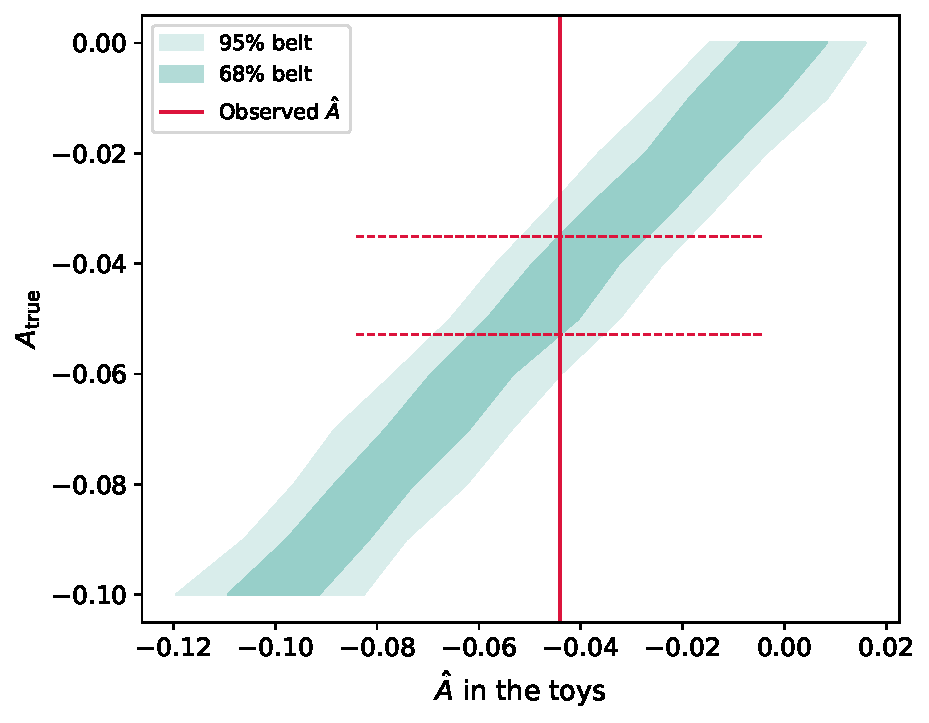
\includegraphics[width=\columnwidth]{figures/validation_neyman_belt.pdf}
\caption{Confidence belt of $\hat A$ from toy-MC experiments (central $68\%$ and $95\%$ ranges) as a function of $A_{\mathrm{true}}$; the vertical line is the observed $\hat A$ and the dashed lines the resulting $68\%$ interval.}
\label{fig:checks_belt}
\end{figure}

The detection asymmetry of kaons depends on their momentum; as a direct check, the joint fit was repeated in three bins with equal numbers of candidates of the transverse momentum $p_T$ and of the momentum $p$ of the $B$ candidate (Table~\ref{tab:checks_momentum}): the three values are compatible with the global one, with a largest deviation of $1.4\sigma$.

\begin{table}[h]
\centering
\begin{tabular}{lccc}
\toprule
Bin & range [GeV] & $n$ & $\Araw$ \\
\midrule
$p_T$, 1 & $1.0$--$4.7$ & $6577$ & $-0.0563\pm0.0169$ \\
$p_T$, 2 & $4.7$--$8.2$ & $6577$ & $-0.0362\pm0.0141$ \\
$p_T$, 3 & $8.2$--$30.5$ & $6577$ & $-0.0452\pm0.0134$ \\
$p$, 1 & $26.7$--$78.1$ & $6577$ & $-0.0391\pm0.0139$ \\
$p$, 2 & $78.1$--$110.1$ & $6577$ & $-0.0475\pm0.0149$ \\
$p$, 3 & $110.1$--$288.5$ & $6577$ & $-0.0478\pm0.0153$ \\
\bottomrule
\end{tabular}
\caption{$\Araw$ (joint Frequentist fit) in terciles of the transverse momentum and of the momentum of the $B$ candidate.}
\label{tab:checks_momentum}
\end{table}

The values of Table~\ref{tab:checks_momentum} are plotted in Fig.~\ref{fig:momentum_terciles} against the global result: no trend with $p_T$ or $p$ is visible.

\begin{figure*}[t]
\centering
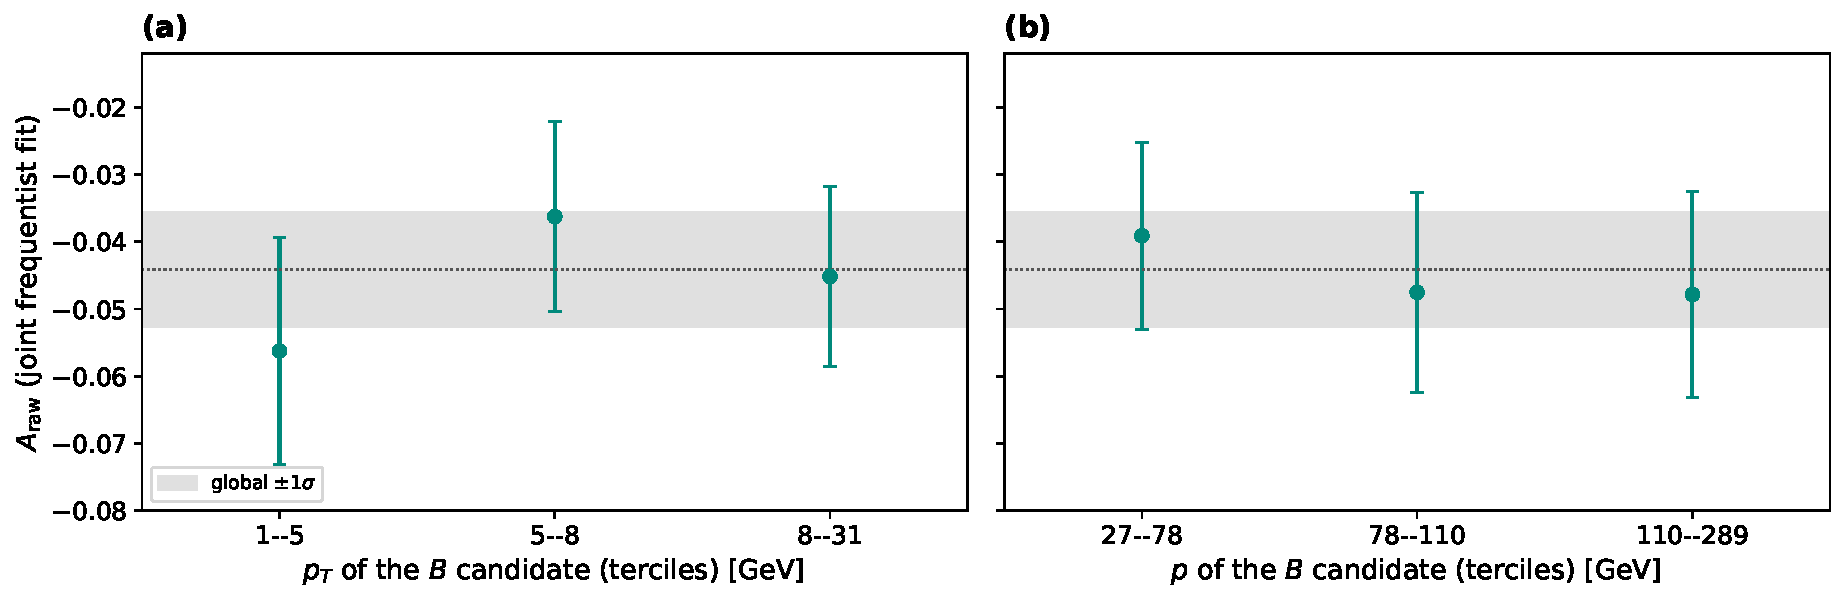
\includegraphics[width=0.85\textwidth]{figures/momentum_terciles.pdf}
\caption{$\Araw$ (joint Frequentist fit) in terciles of (a) the transverse momentum and (b) the momentum of the $B$ candidate, with the global value and its $\pm1\sigma$ band; each bin has $6577$ candidates.}
\label{fig:momentum_terciles}
\end{figure*}

\subsection{Uncertainties of the Twelve Parameters by Three Methods}
\label{sec:checks_covariance}
\emph{In short: the inverse of the Fisher information (Hesse), the bootstrap of the data and the posterior give the same standard deviations for $A$, $A_b$, $\mu$ and $\sigma$; the bootstrap differs for the two yields, because it keeps the total number of candidates fixed, and for the steep slope $\lambda_1^+$, which is weakly constrained.}
The covariance of the fit parameters was estimated in three ways (Table~\ref{tab:checks_covariance}): the inverse of the matrix of second derivatives of $-\ln L$ at the minimum (Hesse), $300$ bootstrap replicas of the data, each refitted, and the posterior sample. The posterior agrees with Hesse to $10\%$ for all the parameters, and the bootstrap does for $A$, $A_b$, $\mu$, $\sigma$ and the other shape parameters. The exceptions of the bootstrap are the steep slope of the $B^+$ background, $\lambda_1^+$ ($0.0057$ against $0.0077$, a weakly constrained and non-parabolic direction, Sec.~\ref{sec:checks_multistart}), and the signal and background yields, $\sigma(N_s)=133$ (Hesse) and $72$ (bootstrap): a resampling of $N$ candidates keeps the total yield fixed, which the extended likelihood does not, and the yields of the bootstrap show the anticorrelated fluctuation of the binomial split; the asymmetry $A$ is not affected. The correlation between $A$ and $A_b$ is $-0.16$, $-0.17$ and $-0.17$ in the three methods.

\begin{table}[h]
\centering
\begin{tabular}{lccc}
\toprule
Parameter & Hesse & Bootstrap & Posterior \\
\midrule
$A$ & $0.0085$ & $0.0085$ & $0.0085$ \\
$A_b$ & $0.0177$ & $0.0183$ & $0.0176$ \\
$N_s$ & $133$ & $72$ & $133$ \\
$N_b$ & $82$ & $72$ & $82$ \\
$\mu$ [MeV] & $0.159$ & $0.159$ & $0.161$ \\
$\sigma$ [MeV] & $0.141$ & $0.150$ & $0.138$ \\
$\lambda_1^+$ & $0.0077$ & $0.0057$ & $0.0078$ \\
$\lambda_2^+$ & $0.00028$ & $0.00030$ & $0.00029$ \\
$f_+$ & $0.028$ & $0.029$ & $0.030$ \\
$\lambda_1^-$ & $0.0047$ & $0.0043$ & $0.0047$ \\
$\lambda_2^-$ & $0.00040$ & $0.00038$ & $0.00039$ \\
$f_-$ & $0.039$ & $0.036$ & $0.037$ \\
\bottomrule
\end{tabular}
\caption{Standard deviation of the parameters of the nominal fit from the Hesse matrix, from the bootstrap of the data and from the posterior.}
\label{tab:checks_covariance}
\end{table}

Figure~\ref{fig:uncertainties_12} shows the same comparison as the ratio to the Hesse uncertainty. The posterior agrees with Hesse within $10\%$ for all parameters; the bootstrap does too, except for the yields (the bootstrap of the data keeps the total number of candidates fixed, which removes the Poisson fluctuation of $N_s$) and $\lambda_1^+$.

\begin{figure*}[t]
\centering
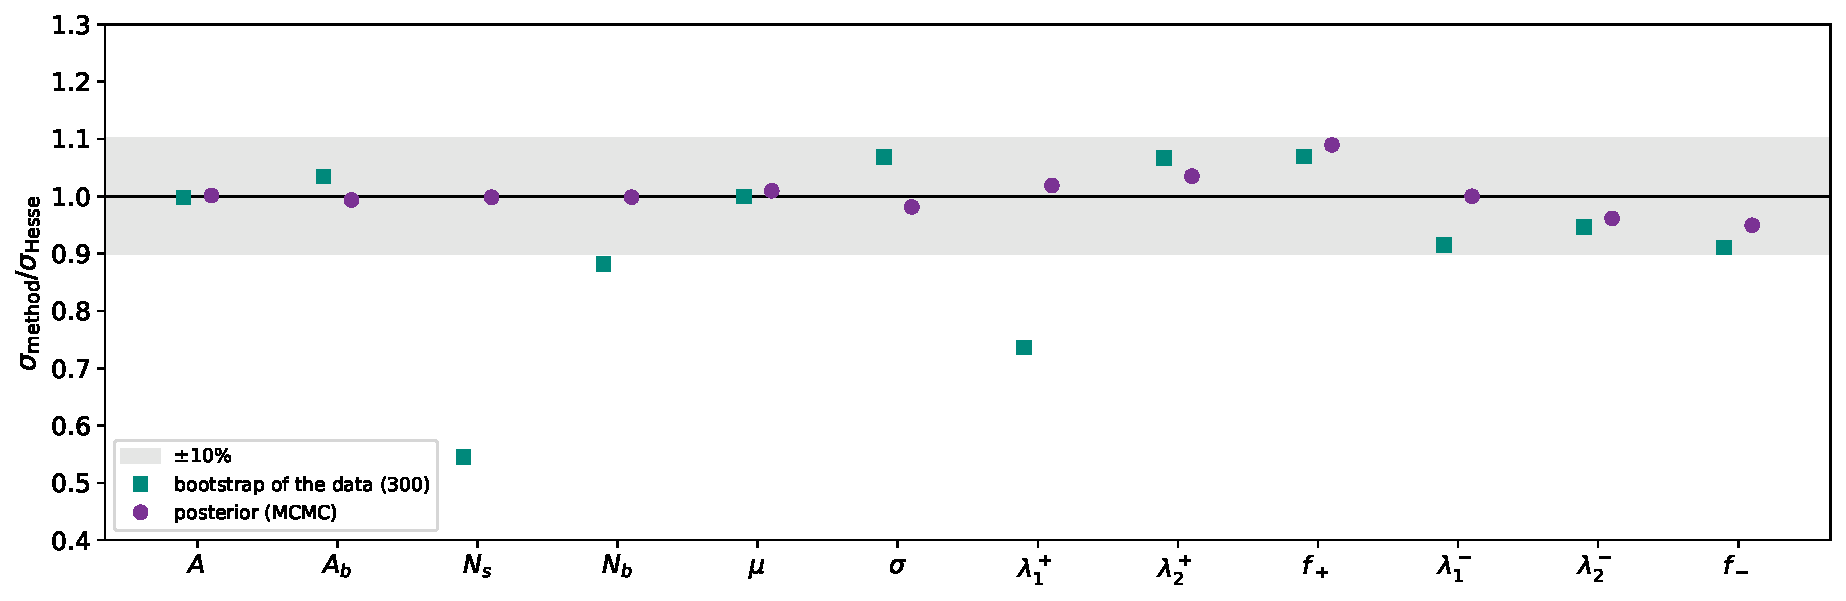
\includegraphics[width=0.85\textwidth]{figures/uncertainties_12.pdf}
\caption{Standard deviation of the twelve parameters of the nominal fit from the bootstrap of the data ($300$ replicas) and from the posterior, divided by the Hesse uncertainty; the band is $\pm10\%$.}
\label{fig:uncertainties_12}
\end{figure*}

\subsection{Starting Values and Weakly Constrained Parameters}
\label{sec:checks_multistart}
\emph{In short: $29$ of $30$ fits from random starting points reach the same minimum; the steep-background fraction is the weakly constrained direction, as the long chain of the Bayesian fit already showed.}
The nominal fit was repeated from $30$ starting points drawn at random (yields and slopes multiplied by a log-normal factor of width $0.5$, the fractions uniform, the asymmetry uniform in $(-0.2,0.2)$): $29$ reach the minimum of the nominal fit ($\hat A=-0.0441$); the remaining one stops in a local minimum $96$ units of $-2\ln L$ above, at $\hat A=-0.052$, which would be rejected by comparing the likelihood values. The profile likelihood of the fraction of the steep component for $B^+$ (the parameter whose chain mixes slowly in the narrow window, Sec.~\ref{sec:bayes_gof}) is asymmetric: $q(f_+)=1$ at $0.085$ and $0.140$ around the best value $0.112$, with a longer tail towards large fractions where the two exponentials exchange their roles. The uncertainty of $A$ does not depend on it (correlation below $0.1$).

\FloatBarrier
